\section{Results}
\label{sec:results}
In this section we describe the results obtained from our simulations. We have simulated two scenarios: A square room where the pedestrians exit through a single door, and pedestrians walking through a corridor where there is a bidirectional flow. For each scenario we describe the parameters we have set for the scenario, which features we found worth measuring for this scenario, the results we expected, and the results we obtained. Possible remedies for any discrepancies between the expected and the actual results are discussed in section~\ref{sec:discussion}.

\subsection{The square room scenario}
In this scenario we simulate pedestrians leaving a square room of 10 m by 10 m with a single $80cm$ wide door. 100 pedestrians are positioned randomly throughout the room. The second the simulation start all pedestrians head for the exit. The parameters for this simulation are as follows:
% TODO: Hints about the constants - do not repeat parameter definitions
\begin{itemize*}
    \item $A: 3,0$, $B: 0,2$, $U: 2.0$, $\lambda: 0,1$.
    \item Mean desired velocity: $1,34 m/s$, deviation $0,26 m/s$. Max velocity factor $1,3$.
    \item Radius mean $0,3 m$, deviation $0,01 m$.
    \item Relaxation time: $1,0 s$.
    \item Number of pedestrians: $100$.
\end{itemize*}

First the claim of the "faster-is-slower" effect is tested.
\begin{quote}
Even counterintuitive
effects are well reproduced. This includes the “faster is-
slower effect” and stripe formation in intersecting flows. \cite{self-org}
\end{quote}
We would then expect that a high nervousness would lead to slower evacuation, because of additional clogging at the doorway. But this phenomena do not occur in our simulation see figure \ref{FastIsSlow}
\begin{figure}
\centering
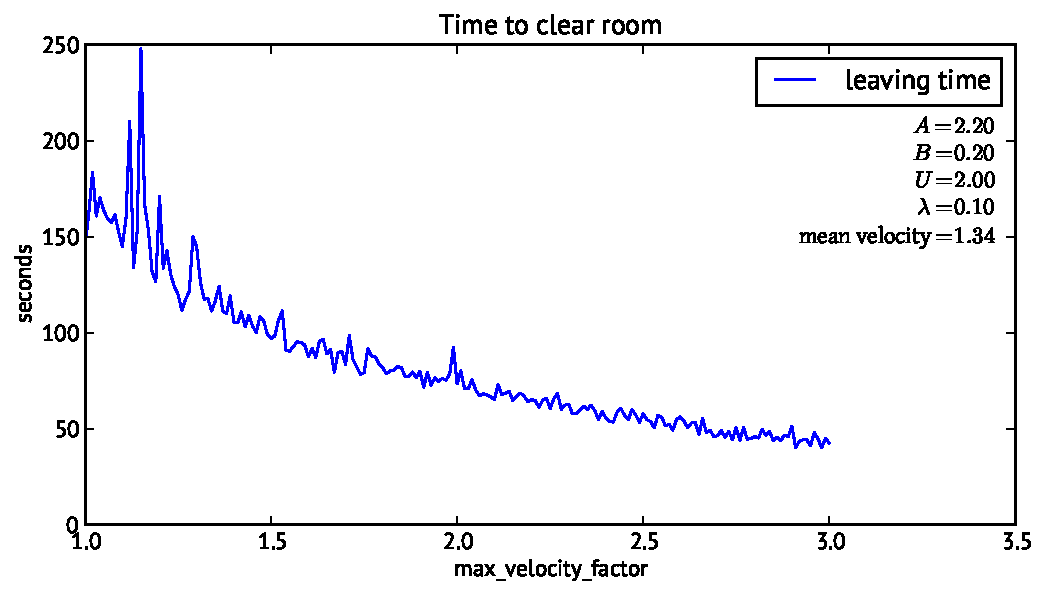
\includegraphics[scale=0.5]{Figures/fastIsSlowNot}
\caption{Fast is not slow}
\label{FastIsSlow}
\end{figure}
The larger the nervousness the faster is the evacuation. We have increased the max-velocity factor sow much that people eventually move through the walls. This start occurring around max-velocity-factor = 2.5, and measurements beyond this point are neglected.

Pedestrian flow rate is measure in the door opening, and the density of pedestrians in a 2 m by 2 m area directly in front of the door is measured. We also measure the time it takes for all pedestrians to leave the room.

The parameters for this simulation are as follows:

% TODO: Add parameters that are varied.


\subsection{The corridor scenario}
In this scenario we simulate pedestrians walking in both directions along a 20 
m long and six metres wide corridor. The pedestrians are divided into two 
groups, starting in opposite ends of the corridor and moving towards each 
other. The targets the pedestrians move towards are set 500 metres to each 
side, to make pedestrians walk in almost a straight line instead of converging 
towards the middle of the corridor. Flow rate is measured in the middle of the 
corridor, as is density. We start out with 100 pedestrians, adding a 
continuous inflow of three pedestrians per second, to simulate people arriving 
from outside the simulated area. Both the initial placement and the inflow of 
pedestrians are distributed randomly (i.e. approximately evenly) between the 
two ends of the corridor.

We expect to see lane formations through out our simulations
and the freezing by heating effect when we start raising the mean velocity
of the agents.

\subsubsection{Intial conditions and relaxation time $1,0$ second}
In the first simulation the parameters are set after \cite{ABconstant} and
\cite{self-org}, to see if we can replecate their simulations and results.
The parameters for this simulation are as follows:

\begin{itemize*}
    \item $A: 3,0$, $B: 0,2$, $U: 2,0$, $\lambda: 0,1$.
    \item Mean desired velocity: $1,34 m/s$, deviation $0,26 m/s$. Max 
        velocity factor $1,3$.
    \item Radius mean $0,3 m$, deviation $0,01 m$.
    \item Relaxation time: $1,0 s$.
    \item Number of pedestrians: $50$ starting, adding $3/s$.
\end{itemize*}

When running the simulation we observe lane formations, and they almost clog up
in the corridor.

\begin{itemize*}
    \item $A: 3,0$, $B: 0,2$, $U: 2,0$, $\lambda: 0,1$.
    \item Mean desired velocity: $1,34 m/s$, deviation $0,26 m/s$. Max 
        velocity factor $4,0$.
    \item Radius mean $0,3 m$, deviation $0,01 m$.
    \item Relaxation time: $1,0 s$.
    \item Number of pedestrians: $50$ starting, adding $3/s$.
\end{itemize*}

When we do a simulation with the max velocity factor set to $4.0$, the clogging
that occurs in the beginning eases up, and the pedestrians relatively fast
get out of the clogging and continuous toward their target. In this simulation
we also observe lane formations.

\begin{figure}[h]
\centering
\subfloat[The figure show the density in corridor when the parameters are set as \cite{ABconstant} and \cite{self-org}.]{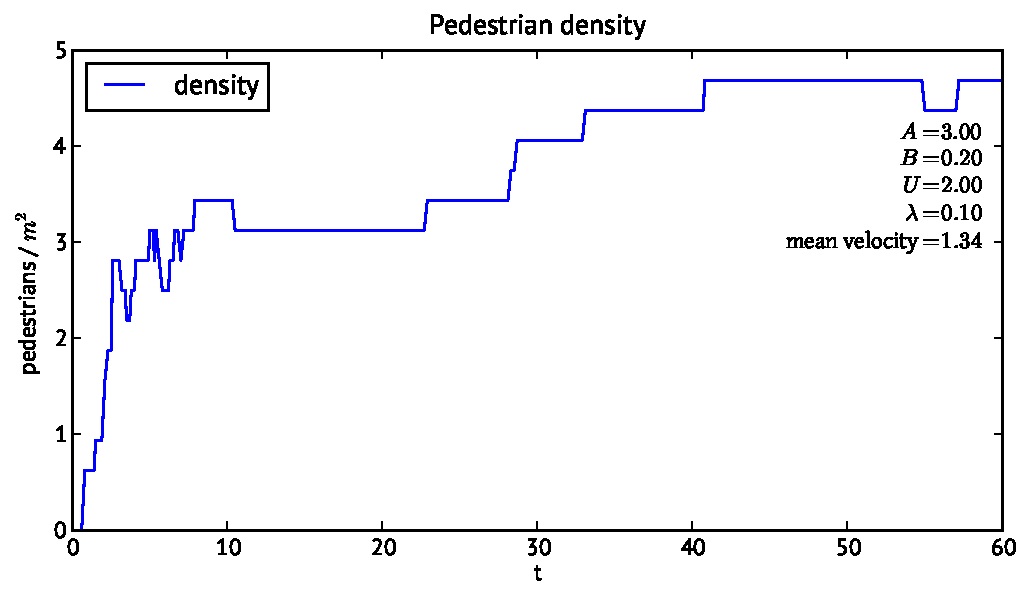
\includegraphics[scale=0.45]{Figures/dens_init_relax1.pdf}}
\subfloat[This figure shows the density in the corridor when the max velocity factor is set to $4.0$, and the other parameters as figure a.]{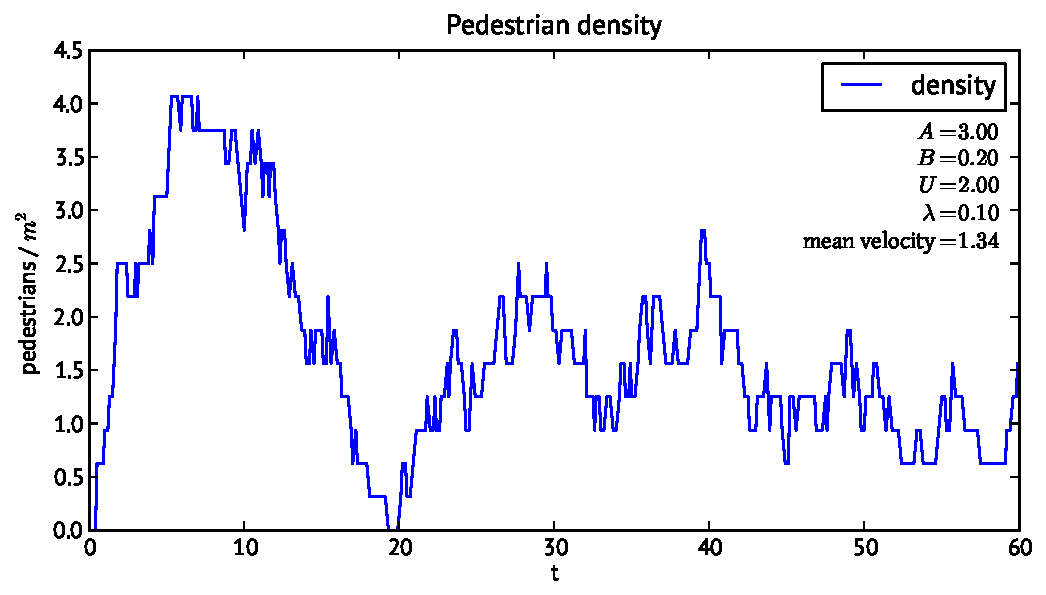
\includegraphics[scale=0.45]{Figures/dens_mvel4_relax1.pdf}}
\caption{These figures was made to see if the freezing by heating effect when raising the max velocity factor. As seen in the figures, the
density does not increase when the max desired velocity is increased. When raising the max desired velocity the density gets lower because
the pedestrians more easely get through the crowd.}
\label{fig:freezingbyheating1}
\end{figure}

\subsubsection{Intial conditions and relaxation time $0,5$ second}
\cite{helbing00} set the relaxation time to $0,5$. As the first corridor simulations we set the parameters as \cite{ABconstant}
and then change the relaxation time to $0,5$ as \cite{helbing00}. After the simulation with the initial conditions, we raise the
max desired velocity to see if we can replicate the freezing by heating effect.

The initial simulation has the following parameters:

\begin{itemize*}
    \item $A: 3,0$, $B: 0,2$, $U: 2,0$, $\lambda: 0,1$.
    \item Mean desired velocity: $1,34 m/s$, deviation $0,26 m/s$. Max 
        velocity factor $1,3$.
    \item Radius mean $0,3 m$, deviation $0,01 m$.
    \item Relaxation time: $0,5 s$.
    \item Number of pedestrians: $50$ starting, adding $3/s$.
\end{itemize*}

The next simulation the parameters are as follows:

\begin{itemize*}
    \item $A: 3,0$, $B: 0,2$, $U: 2,0$, $\lambda: 0,1$.
    \item Mean desired velocity: $1,34 m/s$, deviation $0,26 m/s$. Max 
        velocity factor $4,0$.
    \item Radius mean $0,3 m$, deviation $0,01 m$.
    \item Relaxation time: $0,5 s$.
    \item Number of pedestrians: $50$ starting, adding $3/s$.
\end{itemize*}

When comparing the simulations we do not see the freezing by heating effect.
Instead we see that the pedestrians more easely escape the clogging, and the flow in each directions
gets more steady. In both simulations we observed lane formation.

\begin{figure}[h]
\centering
\subfloat[The figure show the density in corridor when the parameters are set as \cite{ABconstant} and \cite{helbing00}.]{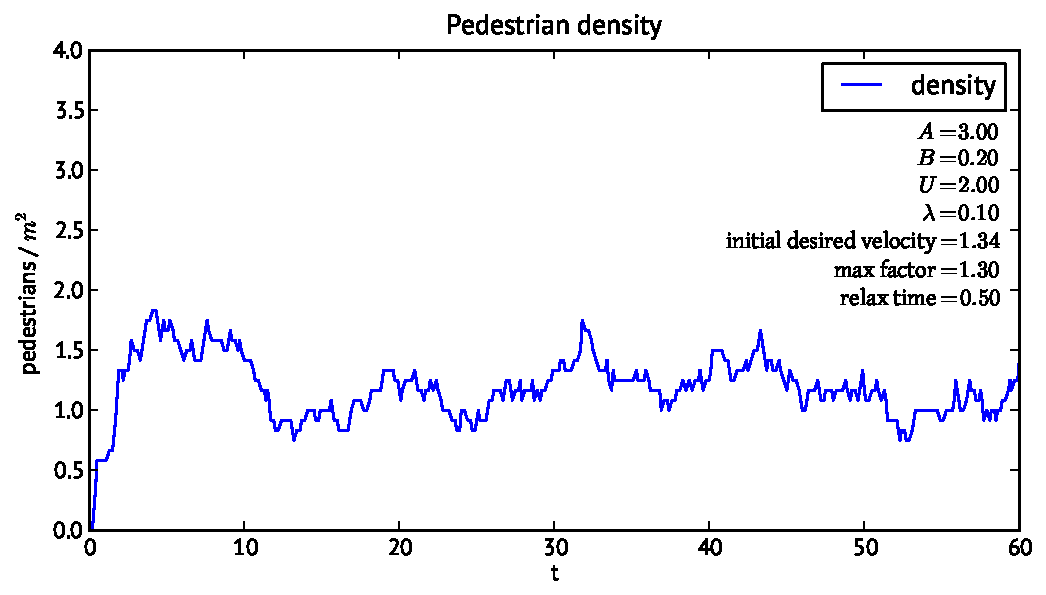
\includegraphics[scale=0.45]{Figures/dens_init_relax05.pdf}}
\subfloat[This figure shows the density in the corridor when the max velocity factor is set to $4.0$ and the max desired velocity is set to $4,0$, and the other parameters as figure a.]{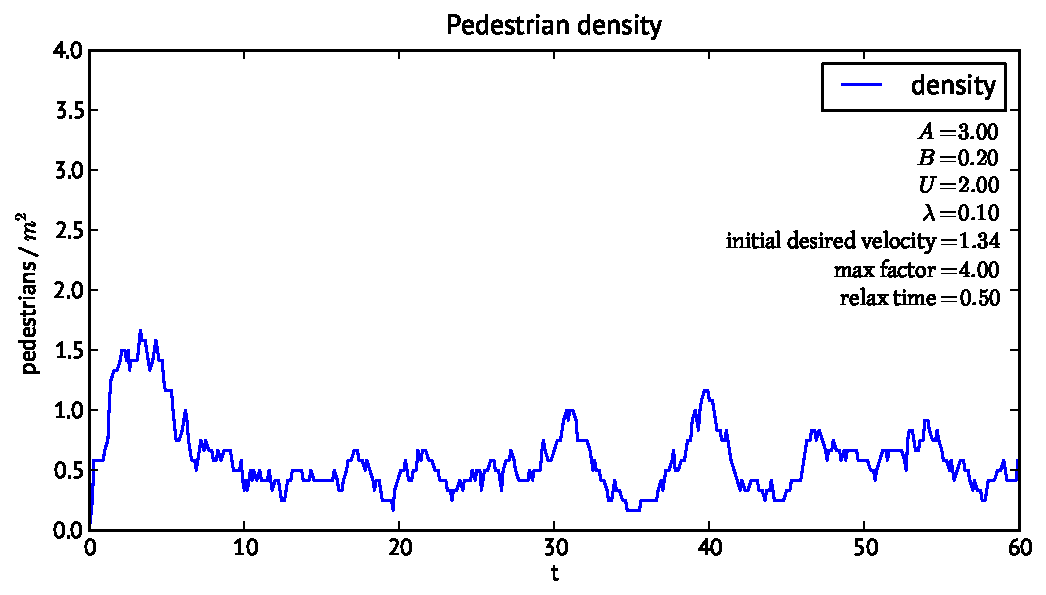
\includegraphics[scale=0.45]{Figures/dens_mvel4_relax05.pdf}}
\caption{These figures was made to see if the freezing by heating effect when raising the max velocity factor. As seen in the figures, the
density does not increase when the max desired velocity is increased. When raising the max desired velocity the density gets lower because
the pedestrians more easely get through the crowd. The difference between figure \ref{fig:freezingbyheating1} and this is the relation time,
respectively $1,0$ and $0,5$.}
\label{fig:freezingbyheating05}
\end{figure}

\subsection{The bottleneck}
In this scenario we wanted to the the oscillitory flows that is reported 
in \cite{self-org} to happen when you have a bidirectional flaw through a 
bottleneck. A print screen from the simulation is shown in figure 
\ref{fig:bottleneckbidirec}.

\begin{figure}[h]
\centering
{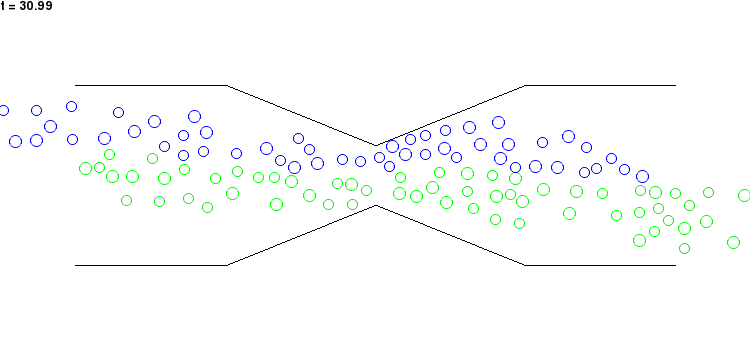
\includegraphics[scale=0.35]{Figures/bottleneck.png}}
\caption{A screen shot of the bottleneck simulation.}
\label{fig:bottleneckbidirec}
\end{figure}

\subsubsection{Attempts to see the faster is slower effect in the bottleneck}
In order to see the faster-is-slower effect we make a series of simulations 
with increasing mean velocity. The results is presented in figure 
\ref{fig:is-faster-slower-in-bottleneck}.

\begin{figure}[h]
\centering
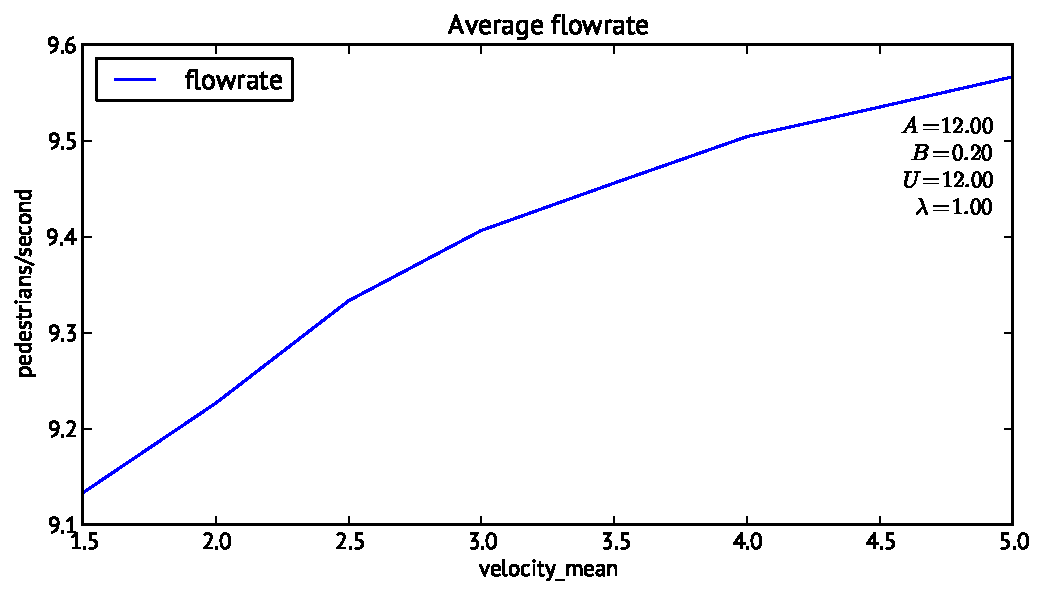
\includegraphics[scale=0.45]{Figures/Wide-kink-one-directional-flowrate-agg.pdf}
\caption{A graph of the flow rate as the average velocity is increased}
\label{fig:is-faster-slower-in-bottleneck}
\end{figure}

\subsection{The corridor with open space}
In this scenario we wanted to reproduce the results that people start to 
clock up in a corridor if there is a sudden area that allow pedestrians to try 
and overtake each other. To see if the flow rate is affected by the pedestrians 
who try to overtake each other we compare the flow rate with the wide space with 
the flow rate from a normal corridor scenario. A screen shot from each simulation 
can be seen in figure \ref{fig:widekink}.

\begin{figure}[h]
\centering
\subfloat[A screen shot of the normal corridor.]{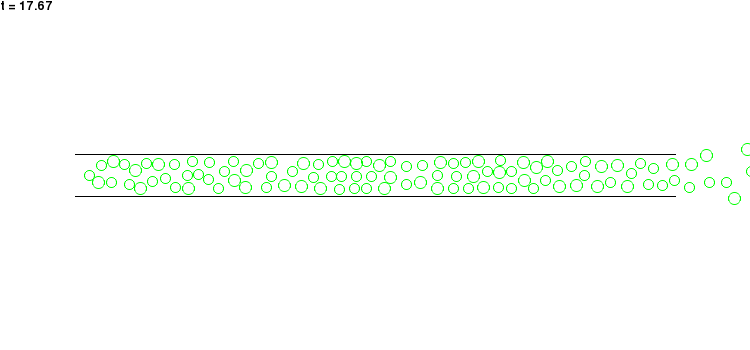
\includegraphics[scale=0.25]{Figures/normalcorridor.png}}
\subfloat[A screen shot of the corridor with a wide space.]{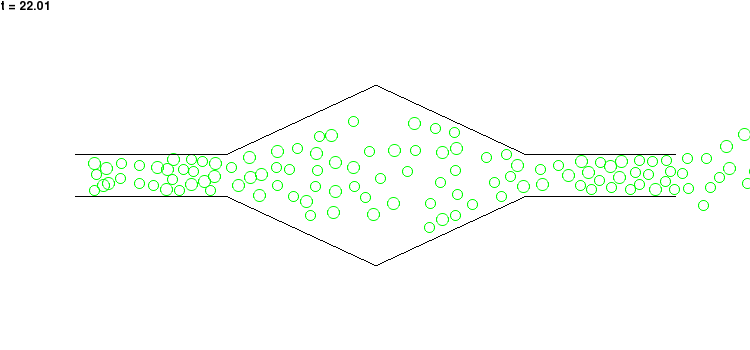
\includegraphics[scale=0.25]{Figures/Widespace.png}}
\caption{The two scenarios we want to compare to see the effect of the wide space.}
\label{fig:chokepoint}
\end{figure}

We expected to see that the flow rate in the scenario shown in figure 
\ref{fig:chokepoint} (b) would be lower than in the scenario (a). What we sat 
in shown in figure \ref{fig:effect-of-widespace}

\begin{figure}[h]
\centering
\subfloat[A graph of the mean velocity of the pedestrians in normal corridor]{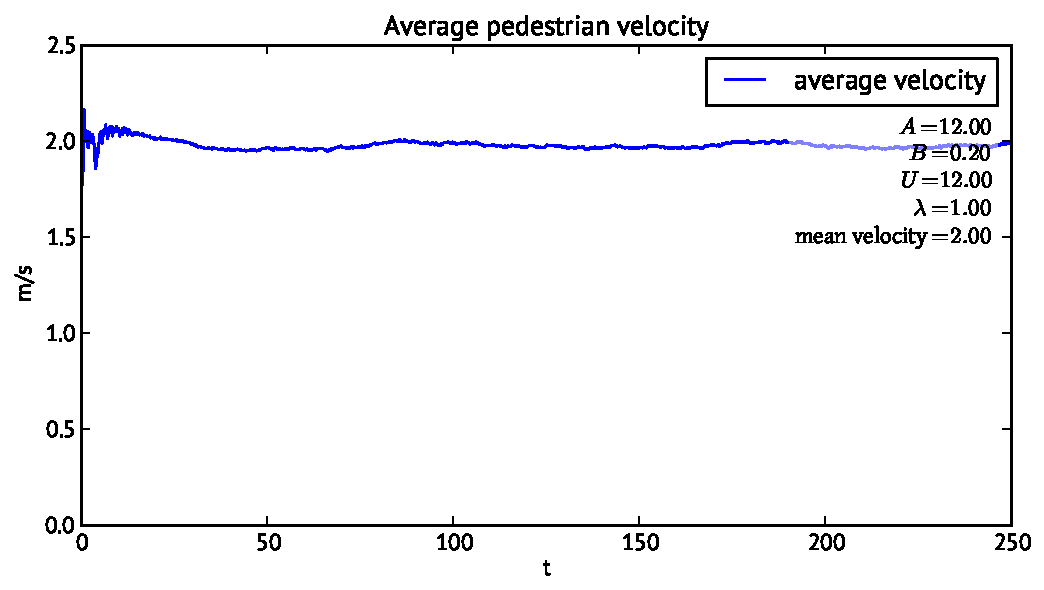
\includegraphics[scale=0.45]{Figures/corridor-velocity.pdf}}
\subfloat[A graph of the mean velocity of the pedestrian in the corridor with a wide space]{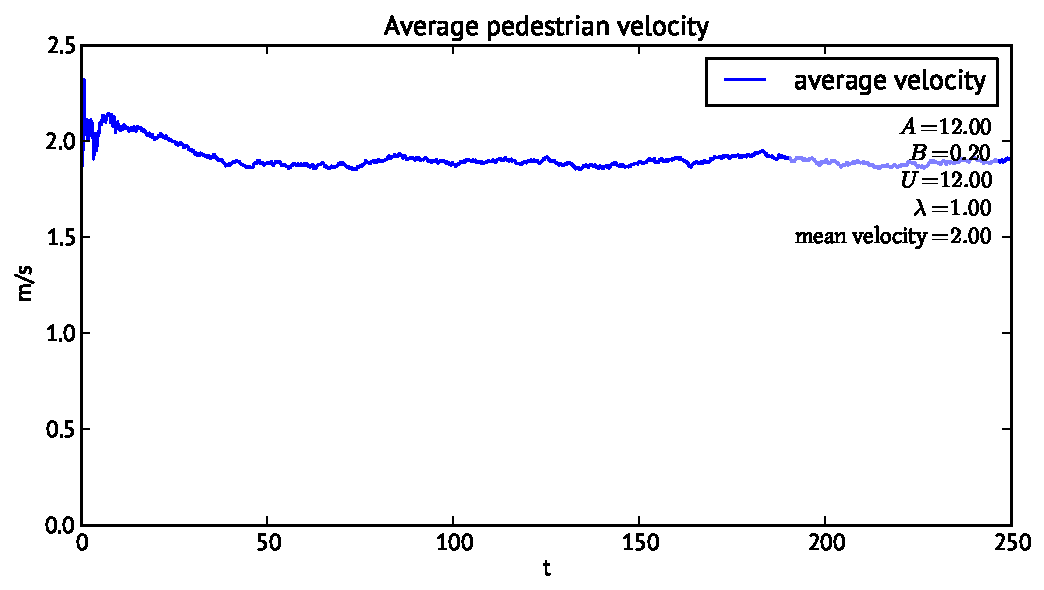
\includegraphics[scale=0.45]{Figures/bottleneck-velocity.pdf}}\\
\subfloat[A graph of the flow rate of the pedestrians in the normal corridor]{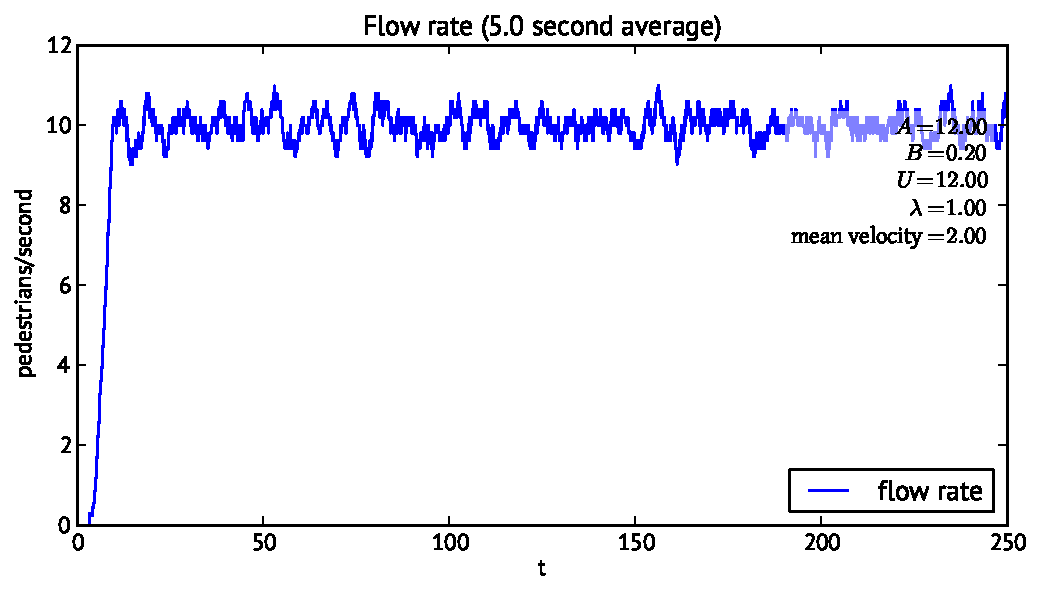
\includegraphics[scale=0.45]{Figures/corridor-flowrate.pdf}}
\subfloat[A graph of the flowrate in the corridor with the wide space]{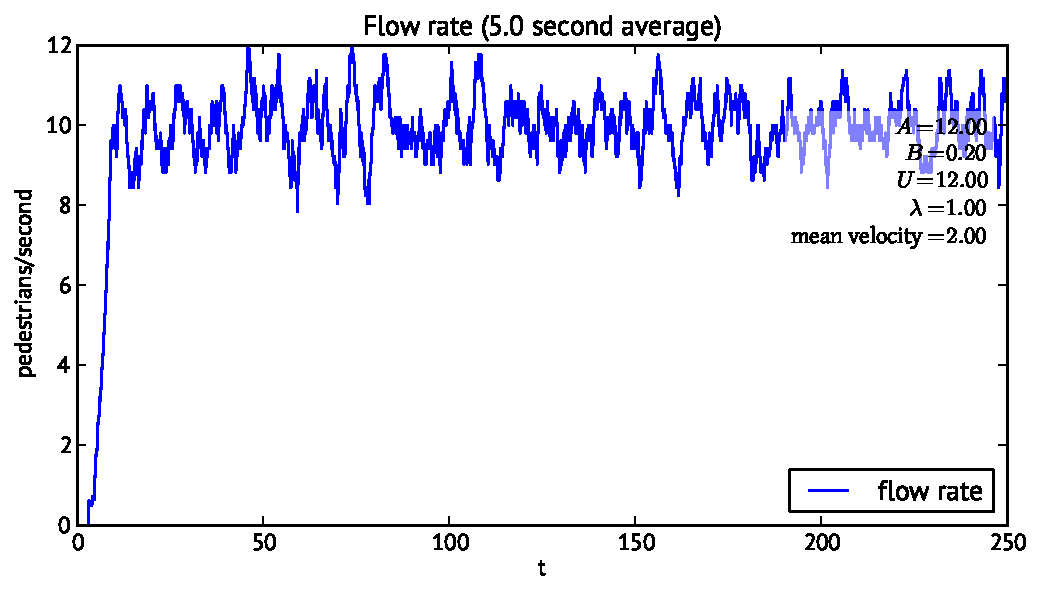
\includegraphics[scale=0.45]{Figures/bottleneck-flowrate.pdf}}
\caption{There is a lowering of the average velocity of the pedestrians due to the bottleneck. We see that there is no consistent lowering of the flowrate due to the bottleneck. What we see is that the flowrate is varying more over time.}
\label{fig:effect-of-widespace}
\end{figure}

\subsubsection{Attempts to see the faster is slower effect in the corridor with wide space}
The faster is slower effect in not observed in the extent that we would expect from 
the article. However the flow rate does not increase linearly with average velocity. 
 
\begin{figure}[h]
\centering
\subfloat[A graph of the flow rate as the average velocity is increased in the case of one directional pedestrian flow.]{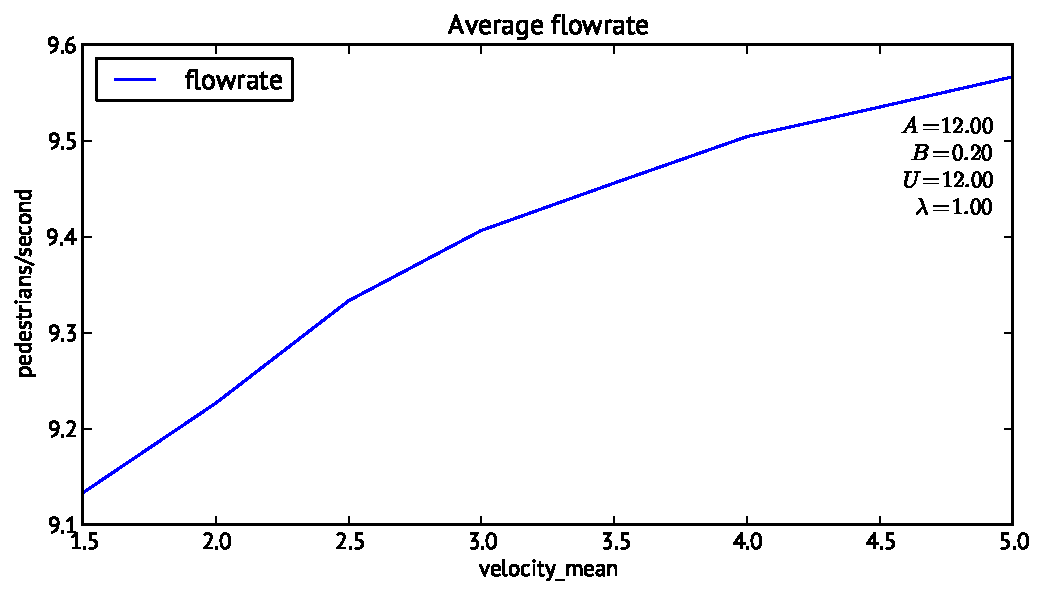
\includegraphics[scale=0.45]{Figures/Wide-kink-one-directional-flowrate-agg.pdf}}
\subfloat[A graph of the flow rate as the average velocity is increased in the case of bidirectional pedestrian flow.]{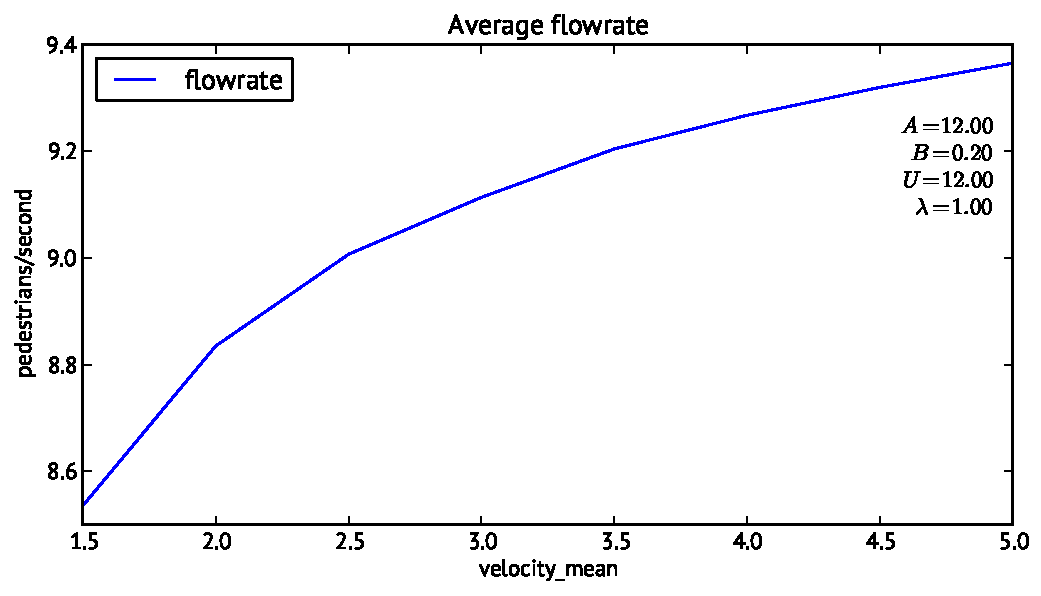
\includegraphics[scale=0.45]{Figures/Widekink-twodirectional-flowrate-agg.pdf}}
\caption{The two scenarios we want to compare to see the effect of the wide space.}
\label{fig:is-faster-slower-in-widekink}
\end{figure}

% TODO: Add parameters that are varied.
